\documentclass[12pt, a4paper]{article}

% Required packages
\usepackage[utf8]{inputenc}
\usepackage[T1]{fontenc}
\usepackage{graphicx}   % For including images
\usepackage{hyperref}   % For clickable links and references
\usepackage{geometry}   % For page margins
\usepackage{amsmath}    % For math formatting
\usepackage{parskip}    % Adds space between paragraphs
\usepackage{float}      % To force image placement with [H]
\usepackage{subcaption} % For side-by-side images (subfigures)

% Page setup
\geometry{margin=1in}

% Document Info
\title{\textbf{Advantages of Fuzzy Clustering for Customer Segmentation}}
\author{Carlo Falchi}
\date{\today}

\begin{document}

\maketitle

\section{Introduction}
Clustering is a fundamental unsupervised machine learning technique used to group similar data points together. In customer segmentation, it helps businesses identify distinct customer groups based on their behavior, preferences, and demographics. Traditional clustering algorithms, such as C-Means, assign each data point to exactly one cluster, a concept known as \textbf{hard clustering}. 
However, in many real-world scenarios, especially in complex domains like e-commerce, customers may exhibit characteristics that belong to multiple segments simultaneously. This is where \textbf{fuzzy clustering}, particularly Fuzzy C-Means (FCM), offers a significant advantage by allowing data points to have partial membership in multiple clusters.
This report will explore the advantages of fuzzy clustering over hard clustering methods, using an e-commerce customer segmentation example based on the provided Python notebook. 
We will compare the results of C-Means and Fuzzy C-Means, highlighting how fuzzy clustering provides a more nuanced and informative understanding of customer behavior.

\section{Data Preparation and Feature Engineering}

In the provided code, the two differents algoirthms were applied to an e-commerce dataset \cite{millat2024ecommerce} to segment customers based on various features such as number of orders, total spending, average order value, and product category preferences.

The dataset contains 10000 orders and 15 different features, it was preprocessed by handling missing values, normalizing numerical features, and encoding categorical variables. Feature engineering was performed to create meaningful attributes that capture customer behavior effectively.

The orders were aggregated by customer ID, in order to get the total number of orders, total spending, average order value, and other relevant metrics for each customer. Other features were created to capture customer preferences for different product categories, device types, and purchase channels.

Finally all the features were scaled using z-score normalization (\cite{scikit-learn}), it standardizes features by removing the mean and scaling them to unit variance. The formula used is: $z = \frac{x - u}{s}$


\section{Hard C-Means Clustering: A Hard Approach}
C-Means is a popular hard clustering algorithm that partitions data into $k$ distinct, non-overlapping clusters. Each data point is assigned to the cluster whose centroid is closest. 
All this type of algorithms are base on an objective function $J$ which **quantifies the quality** of the cluster models and **must be minimized** to obtain optimal cluster.
The algorithm goal is to minimize the objective function $J$. For the hard C-Means this function is the sum of squared distances between each data point and the center of the cluster it belong to.

$$J_h(X,U_h,C) = \sum^c_{i=1}\sum^n_{j=1} u_{ij} 
d^2_{ij}$$


% FIGURE: C-Means PCA
\begin{figure}[H]
    \centering
    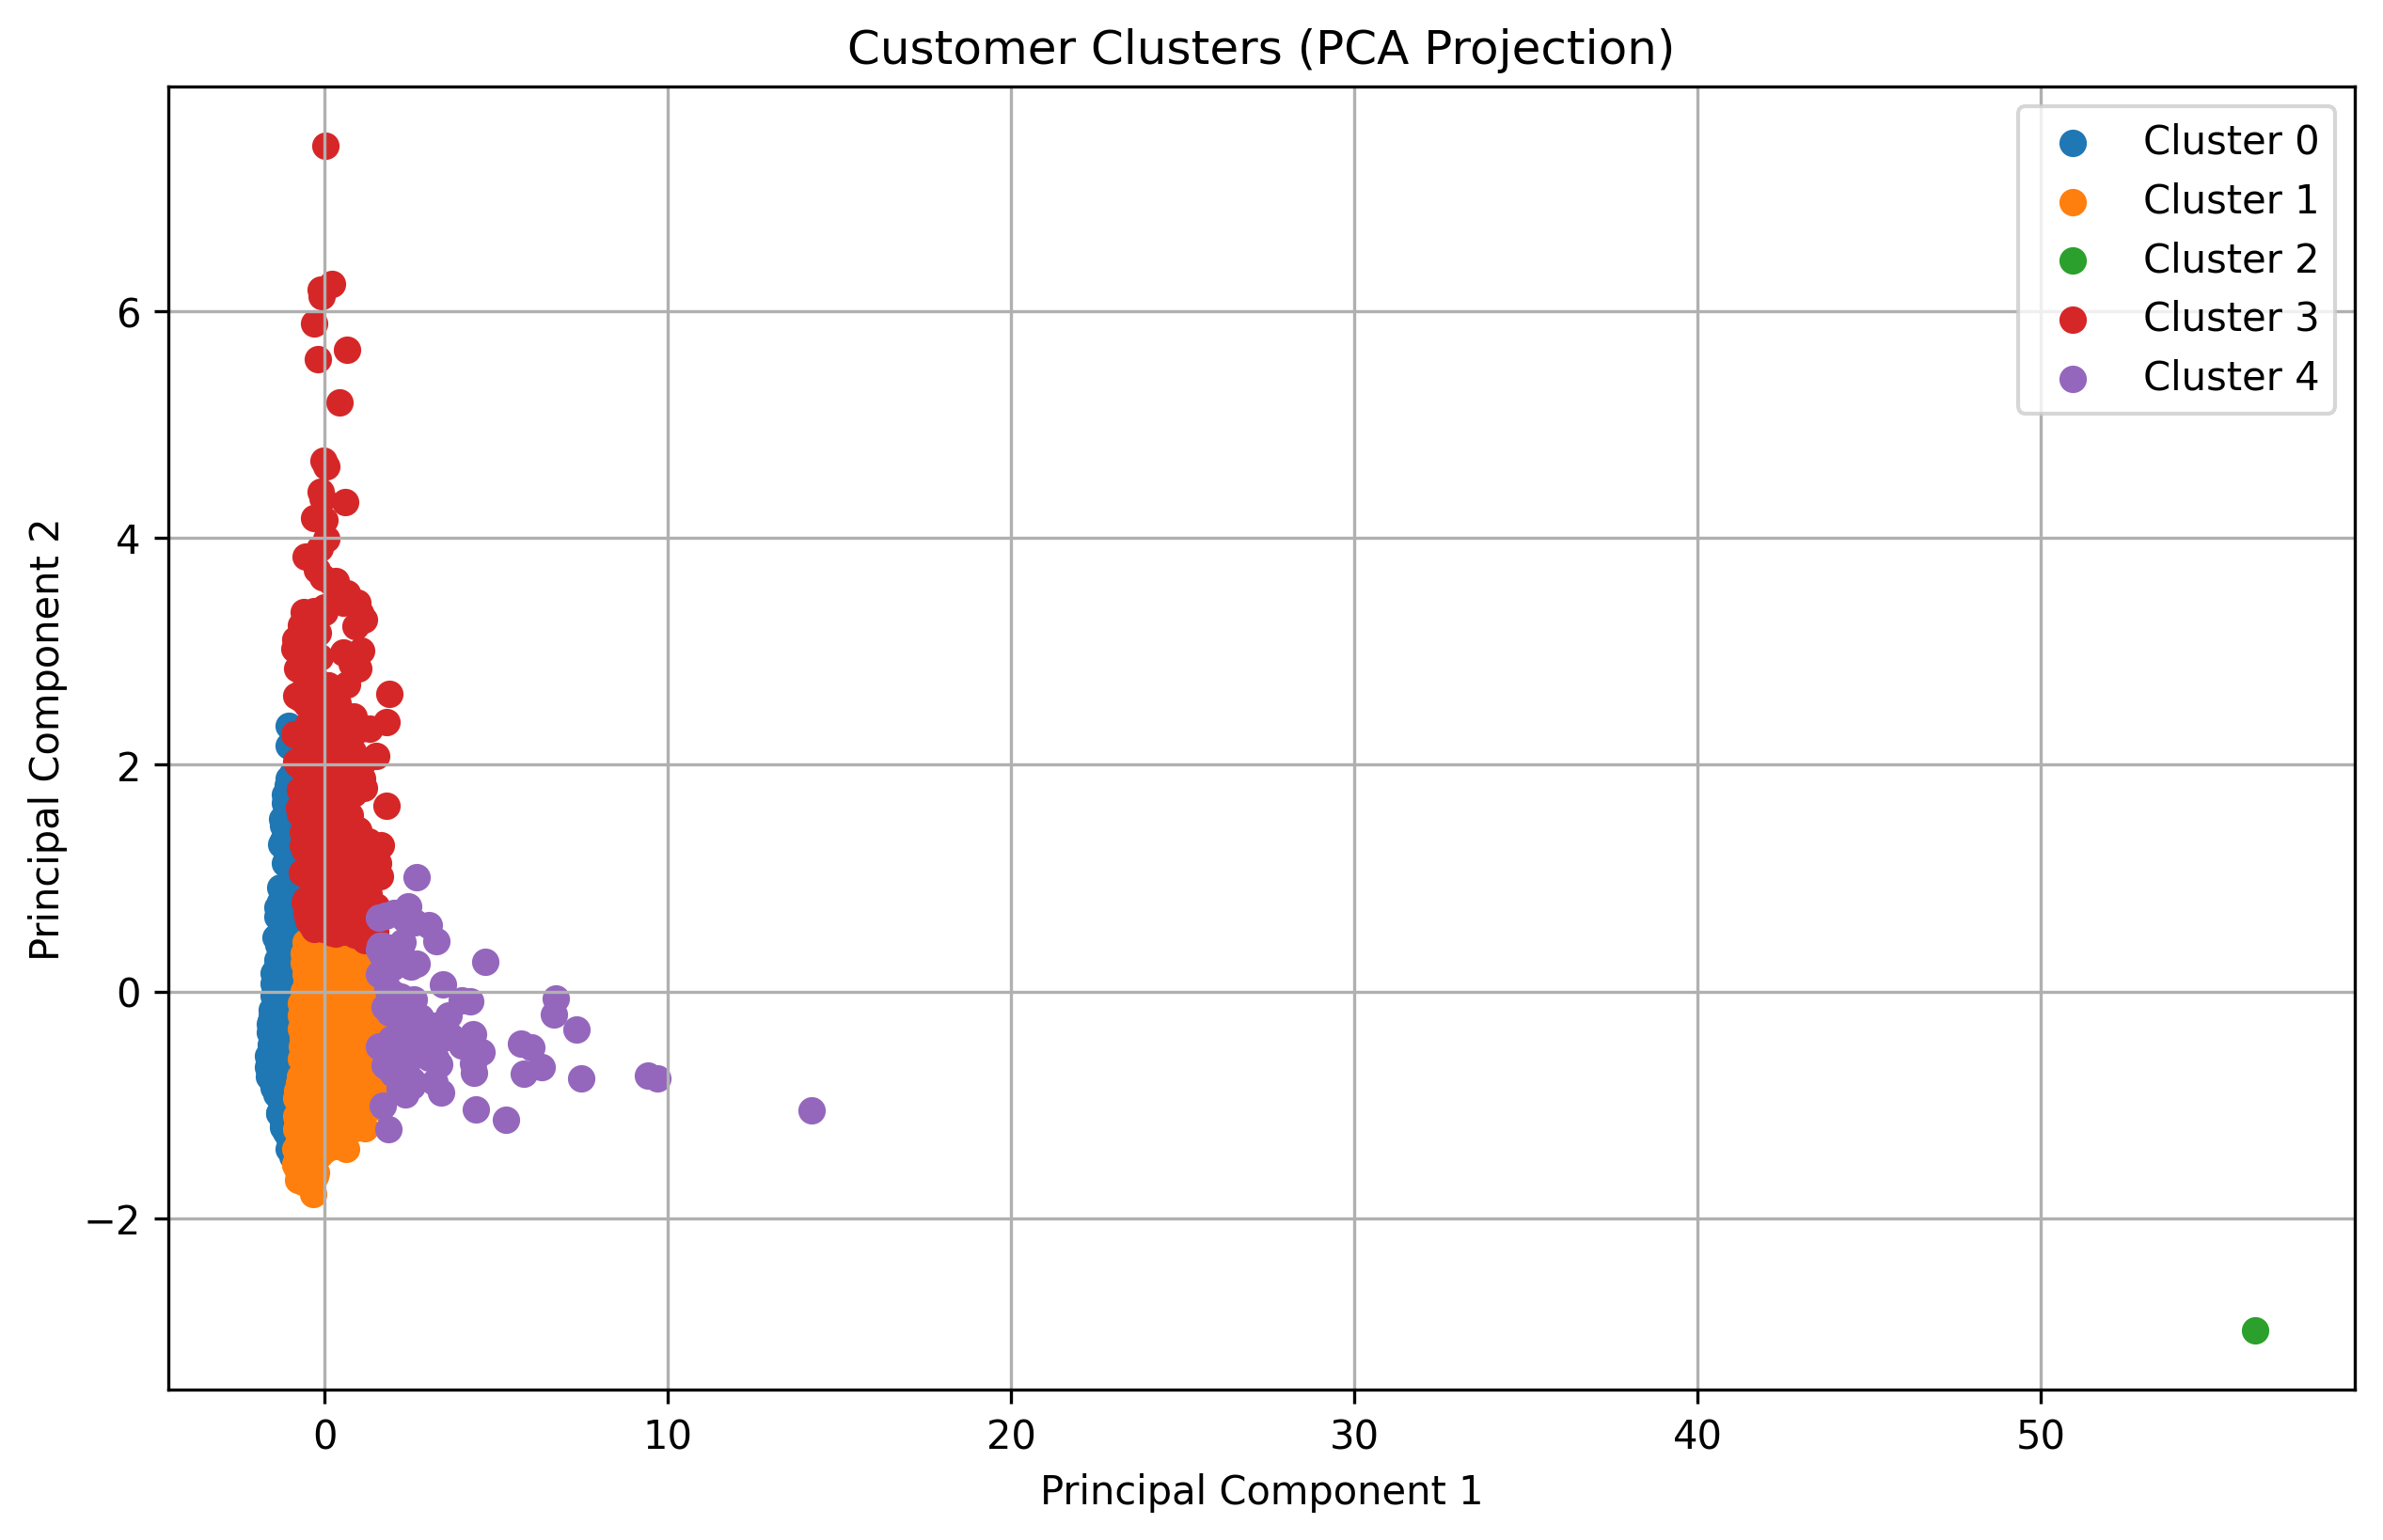
\includegraphics[width=0.85\textwidth]{charts/pca_customer_cluster_hard.png}
    \caption{C-Means Clusters projected onto Principal Components. Note how every customer is forced into a single color (cluster).}
    \label{fig:kmeans_hard}
\end{figure}

\textbf{Limitations of C-Means:}
\begin{itemize}
    \item \textbf{Rigid Assignments}: C-Means forces each data point into a single cluster.
    \item \textbf{Sensitivity to Initial Centroids}: The final clustering result can be sensitive to initialization.
    \item \textbf{Assumption of Spherical Clusters}: C-Means assumes clusters are spherical and equally sized.
\end{itemize}

\section{Fuzzy C-Means Clustering: A Soft Approach}
Fuzzy C-Means (FCM) extends Hard C-Means by allowing data points to belong to multiple clusters with varying degrees of membership. Instead of a binary assignment (0 or 1), FCM assigns a membership value between 0 and 1.

\textbf{Key Advantages:}
\begin{itemize}
    \item \textbf{Handling Overlapping Data:} FCM models real-world ambiguity where customers fit multiple profiles.
    \item \textbf{Robustness to Noise:} Outliers have lower membership weights across clusters, reducing their impact on centroids.
    \item \textbf{Rich Information:} Provides a "membership profile" rather than just a label.
\end{itemize}

The library used in the notebook implements the Fuzzy Probabilistic C-Means algorithm \cite{warner2024scikitfuzzy}, which modifies the objective function to incorporate fuzziness:

$$J_f(X,U_h,C) =\sum_{i=1}^c \sum_{j=1}^n u_{ij}^m \cdot d_{ij}^2$$
Where parameter $m > 1$ determines the fuzziness of the classification, clusters becomes softer/harder with higher/lower value of $m$. 
\section{Experimental Results}

\subsection{Model Evaluation and Parameter Selection}
Before analyzing the clusters, we evaluated the optimal number of clusters ($k$) and the fuzziness parameter ($m$).

The C-Means evaluation (Figure \ref{fig:metrics}a) suggests that $k=5$ is a reasonable choice, showing a balance between the Elbow method and Silhouette scores. For Fuzzy C-Means (Figure \ref{fig:metrics}b), the Fuzzy Partition Coefficient (FPC) decreases as clusters increase, which is typical, but we selected parameters to align with the interpretable groups found in C-Means.

% FIGURE: Side-by-side Metrics
\begin{figure}[H]
    \centering
    \begin{subfigure}[b]{0.48\textwidth}
        \centering
        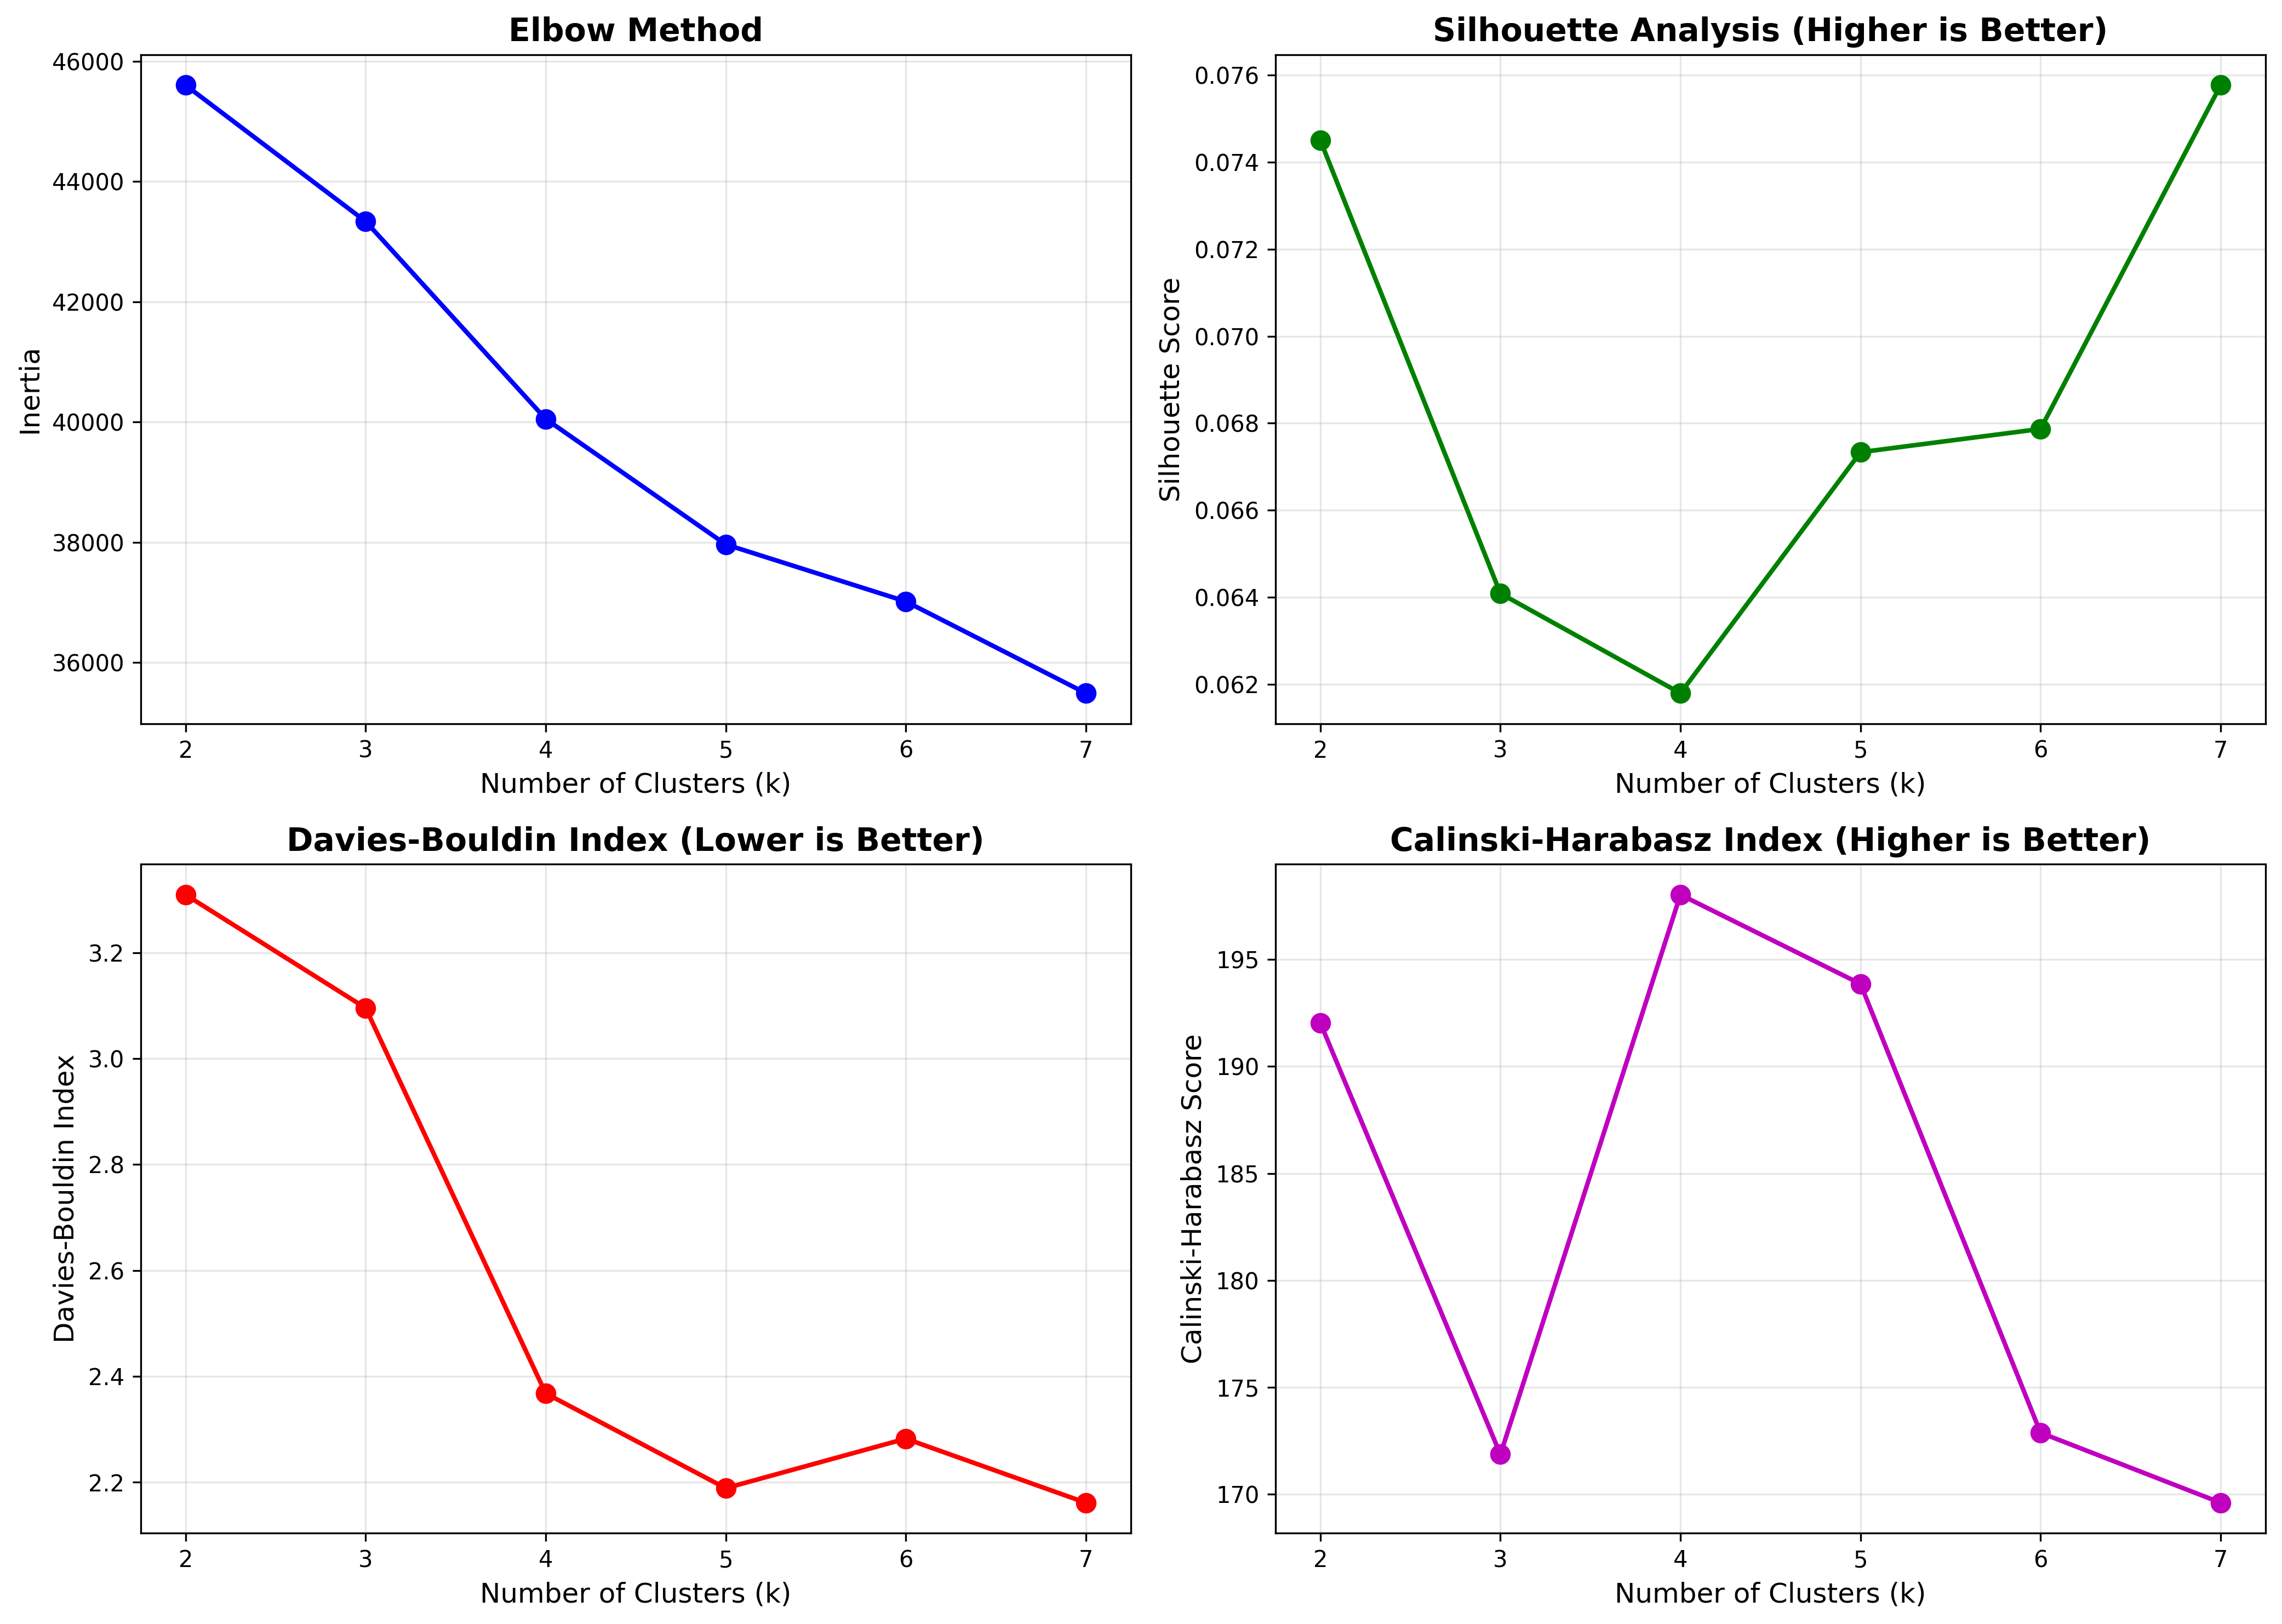
\includegraphics[width=\textwidth]{charts/cluster_evaluation_metrics.png}
        \caption{C-Means Metrics}
    \end{subfigure}
    \hfill
    \begin{subfigure}[b]{0.48\textwidth}
        \centering
        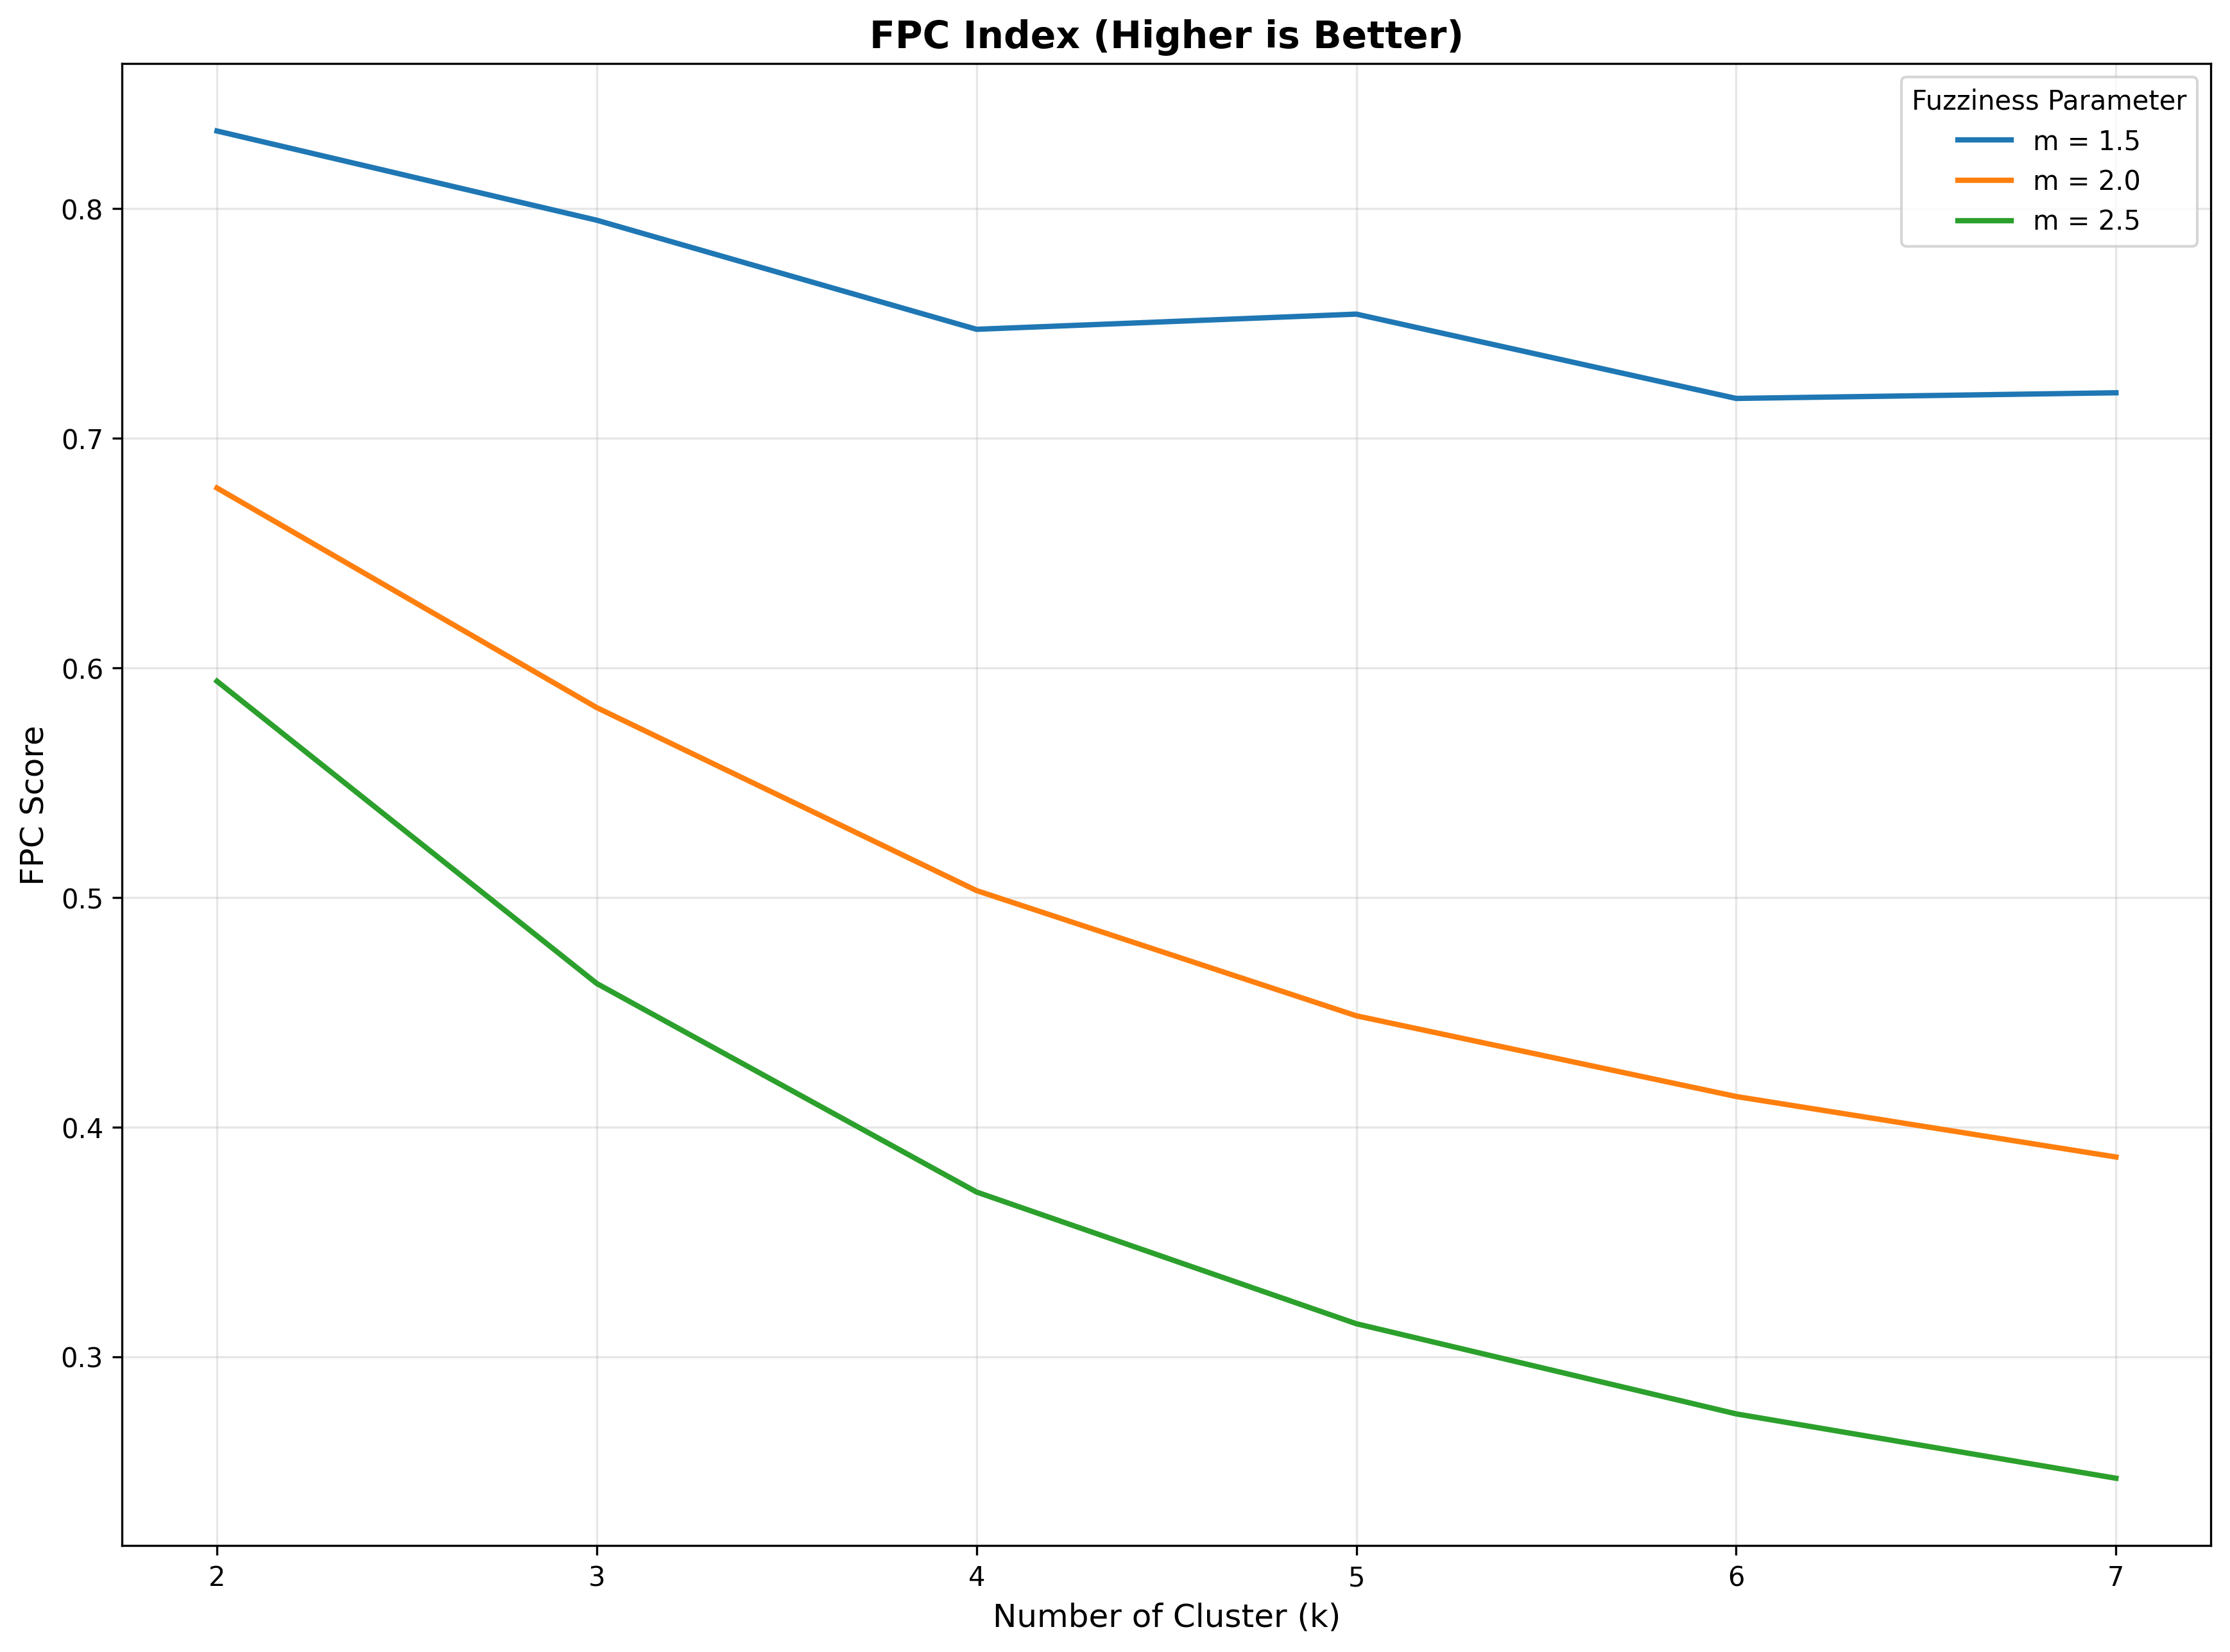
\includegraphics[width=\textwidth]{charts/fuzzy_cluster_evaluation_metrics.png}
        \caption{Fuzzy FPC Scores}
    \end{subfigure}
    \caption{Evaluation metrics used to determine the optimal number of clusters.}
    \label{fig:metrics}
\end{figure}

\subsection{Visualizing Transitional Customers}
While C-Means portrays clusters as distinct islands (see Figure \ref{fig:kmeans_hard}), Fuzzy C-Means reveals the "transitional" nature of customers. In Figure \ref{fig:transitional}, the color scale represents uncertainty. Yellow points indicate customers with high uncertainty (low max membership), meaning they sit between clusters.

% FIGURE: Transitional Customers
\begin{figure}[H]
    \centering
    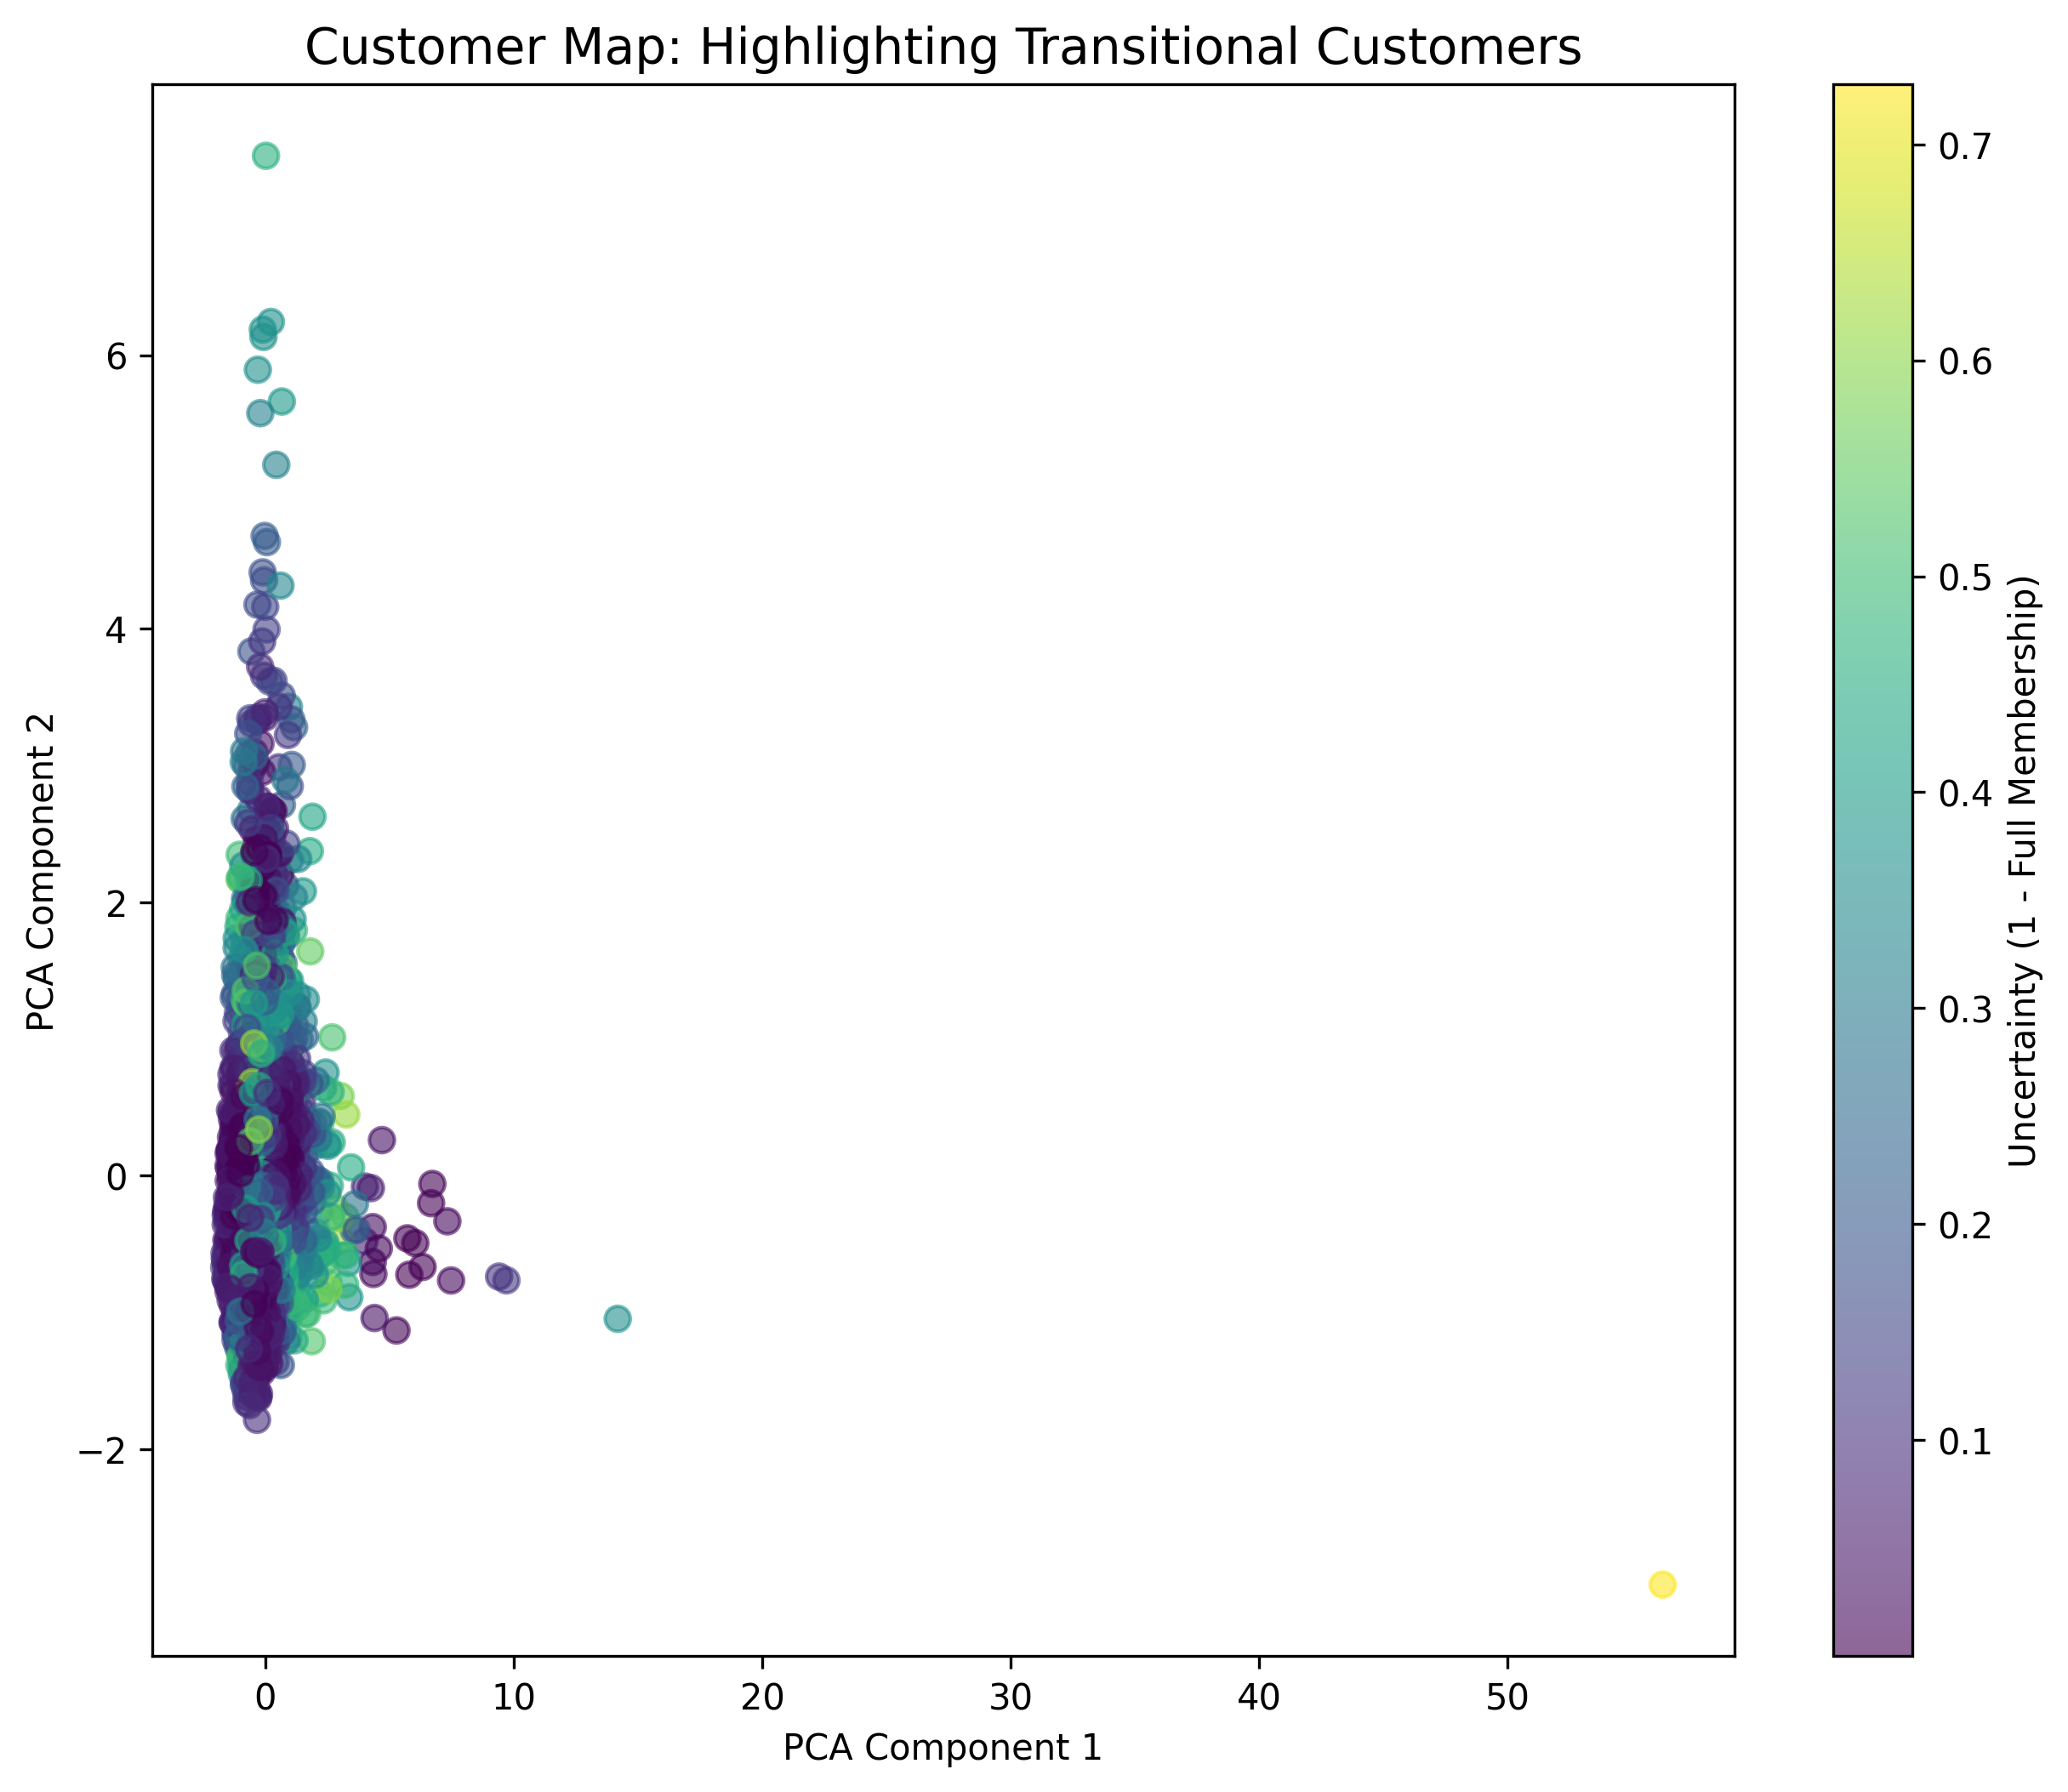
\includegraphics[width=0.85\textwidth]{charts/transinional_customers.png}
    \caption{Fuzzy Clustering Map. Lighter colors (yellow/green) represent "transitional" customers who do not fit neatly into one single segment.}
    \label{fig:transitional}
\end{figure}

\subsection{Membership Certainty Analysis}
The histogram below quantifies how strongly customers belong to their primary cluster. We observe a significant number of customers falling into the "Medium" and "Low" certainty ranges, proving that a hard label would be an oversimplification for these individuals.

% FIGURE: Distribution
\begin{figure}[H]
    \centering
    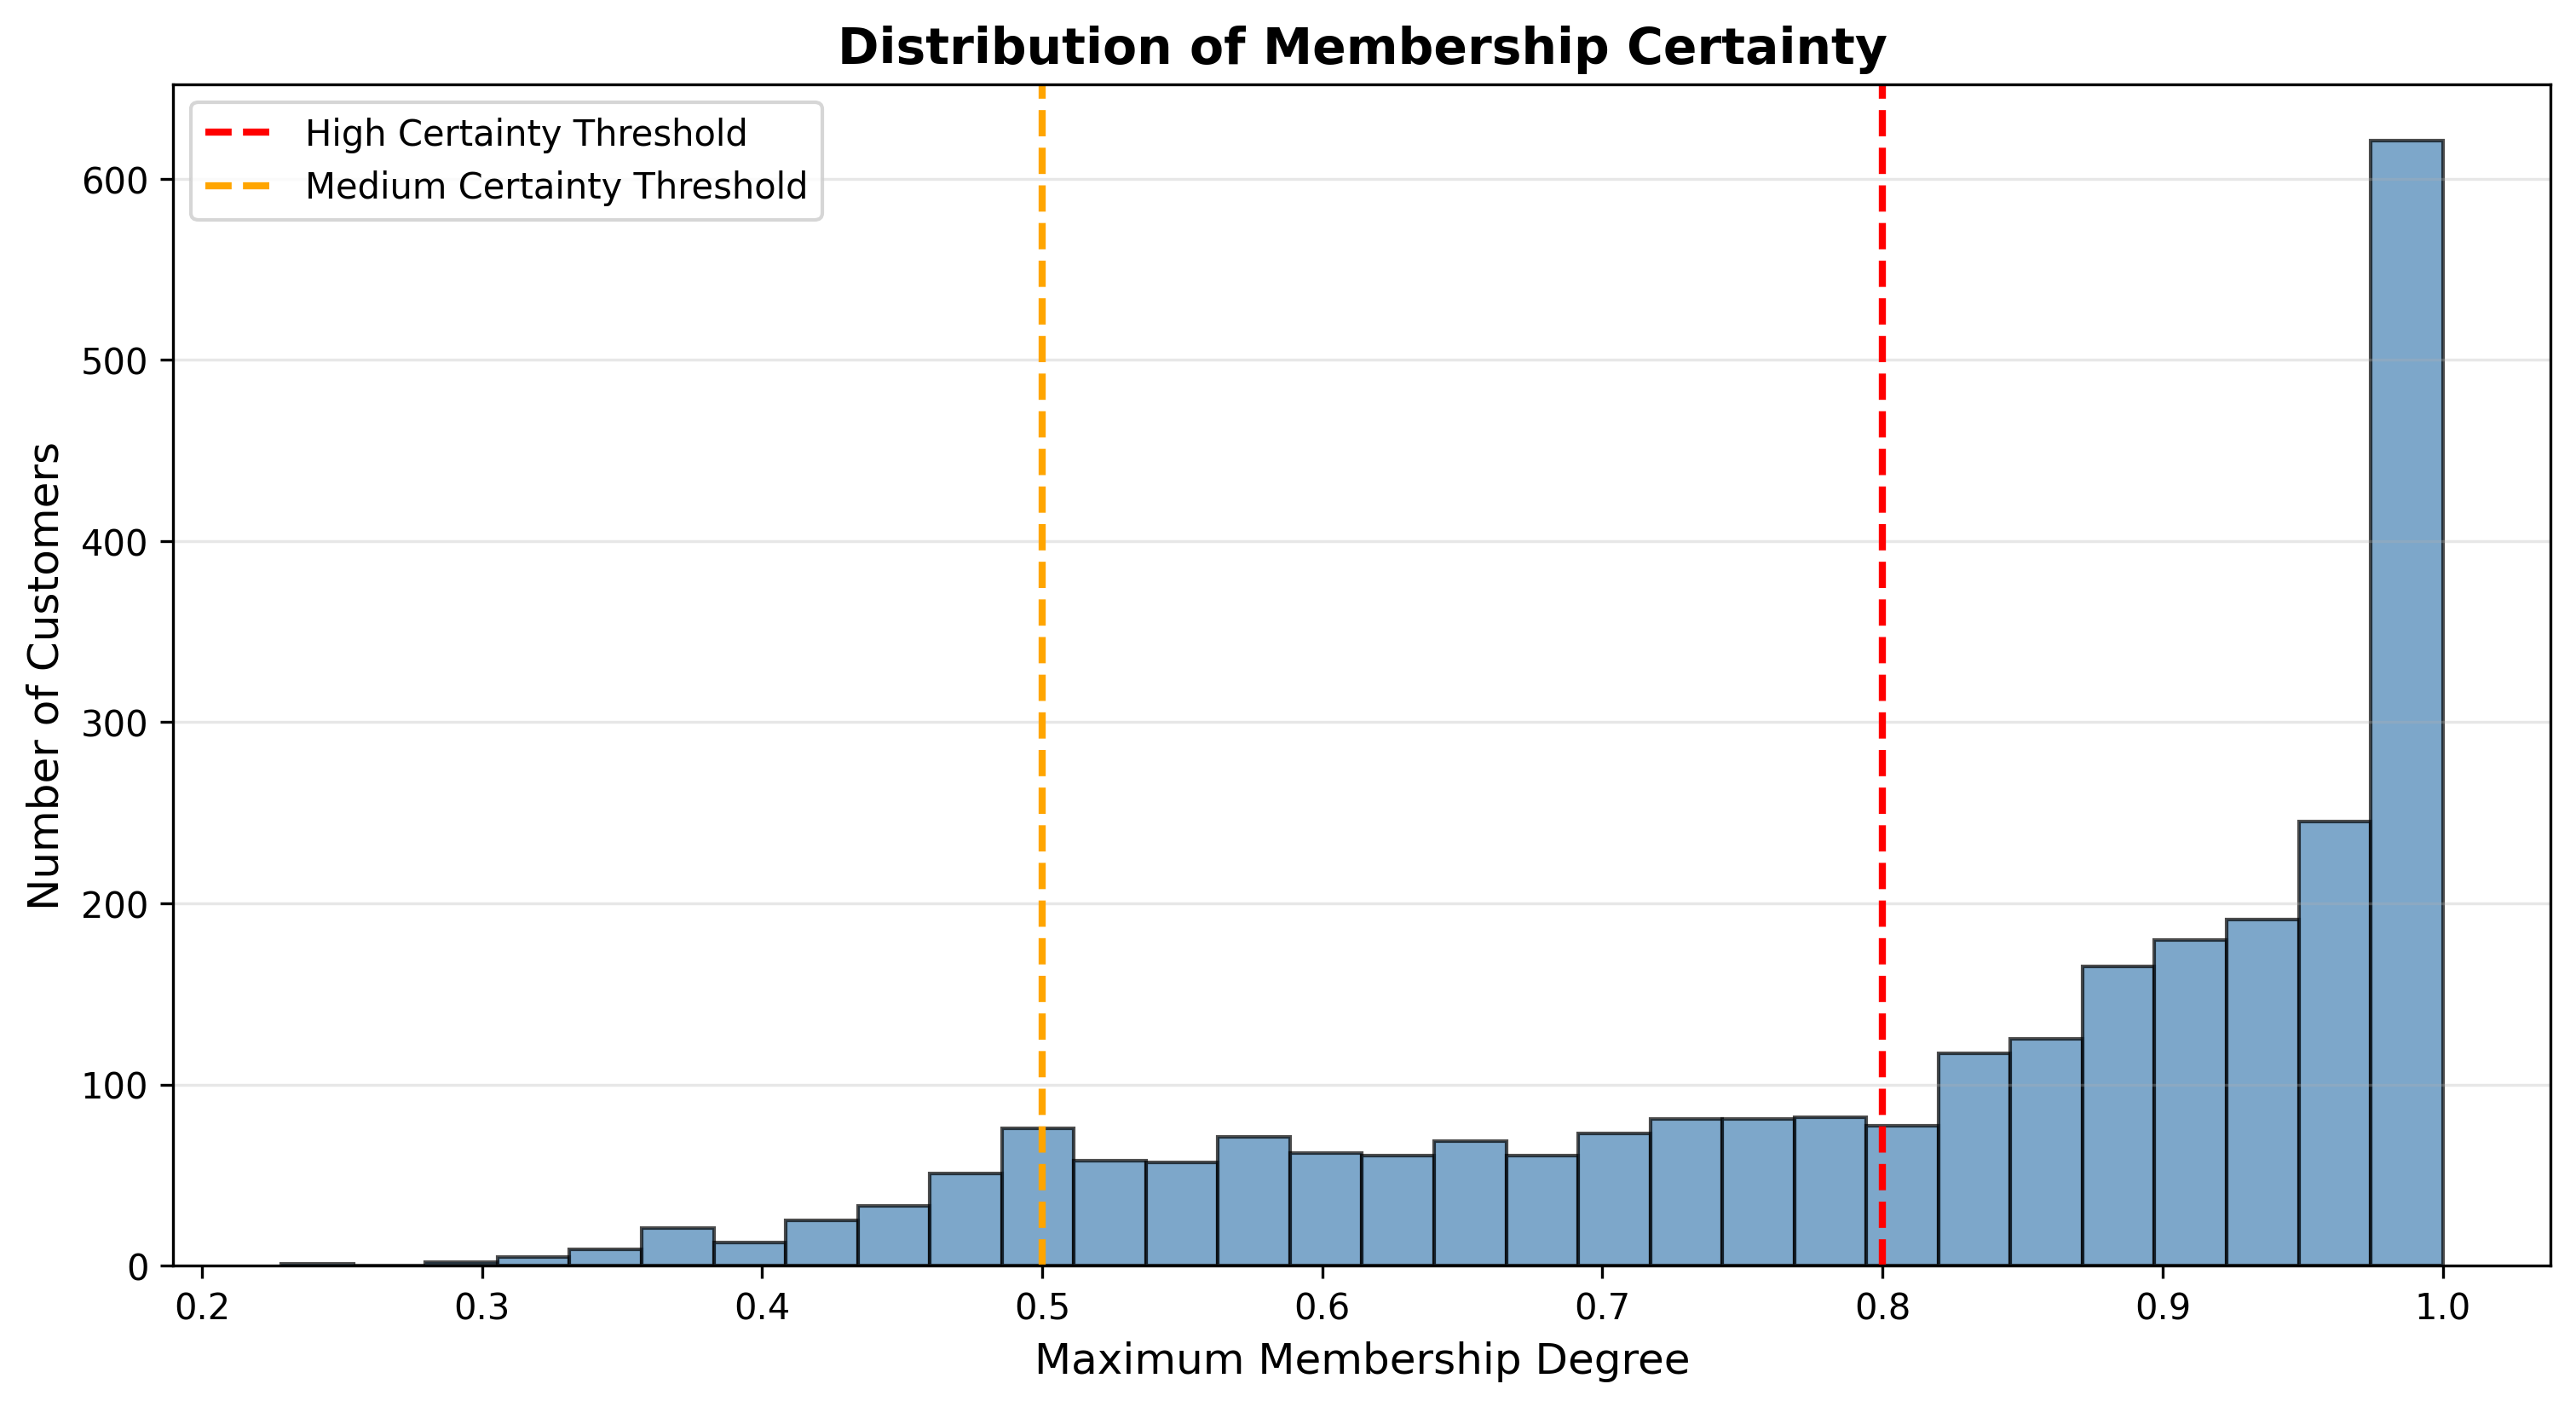
\includegraphics[width=0.9\textwidth]{charts/distribution_membership.png}
    \caption{Distribution of Membership Certainty. The orange and red lines mark thresholds for medium and high certainty.}
    \label{fig:distribution}
\end{figure}

\subsection{Case Study: Hybrid Customers}
To prove the failure of hard labels, we isolated the top 10 most "hybrid" customers. As shown in Figure \ref{fig:hybrid}, these customers have nearly equal probabilities of belonging to multiple clusters (e.g., Cluster 2 and Cluster 3). C-Means would arbitrarily force them into one, losing valuable marketing data.

% FIGURE: Hybrid Customers
\begin{figure}[H]
    \centering
    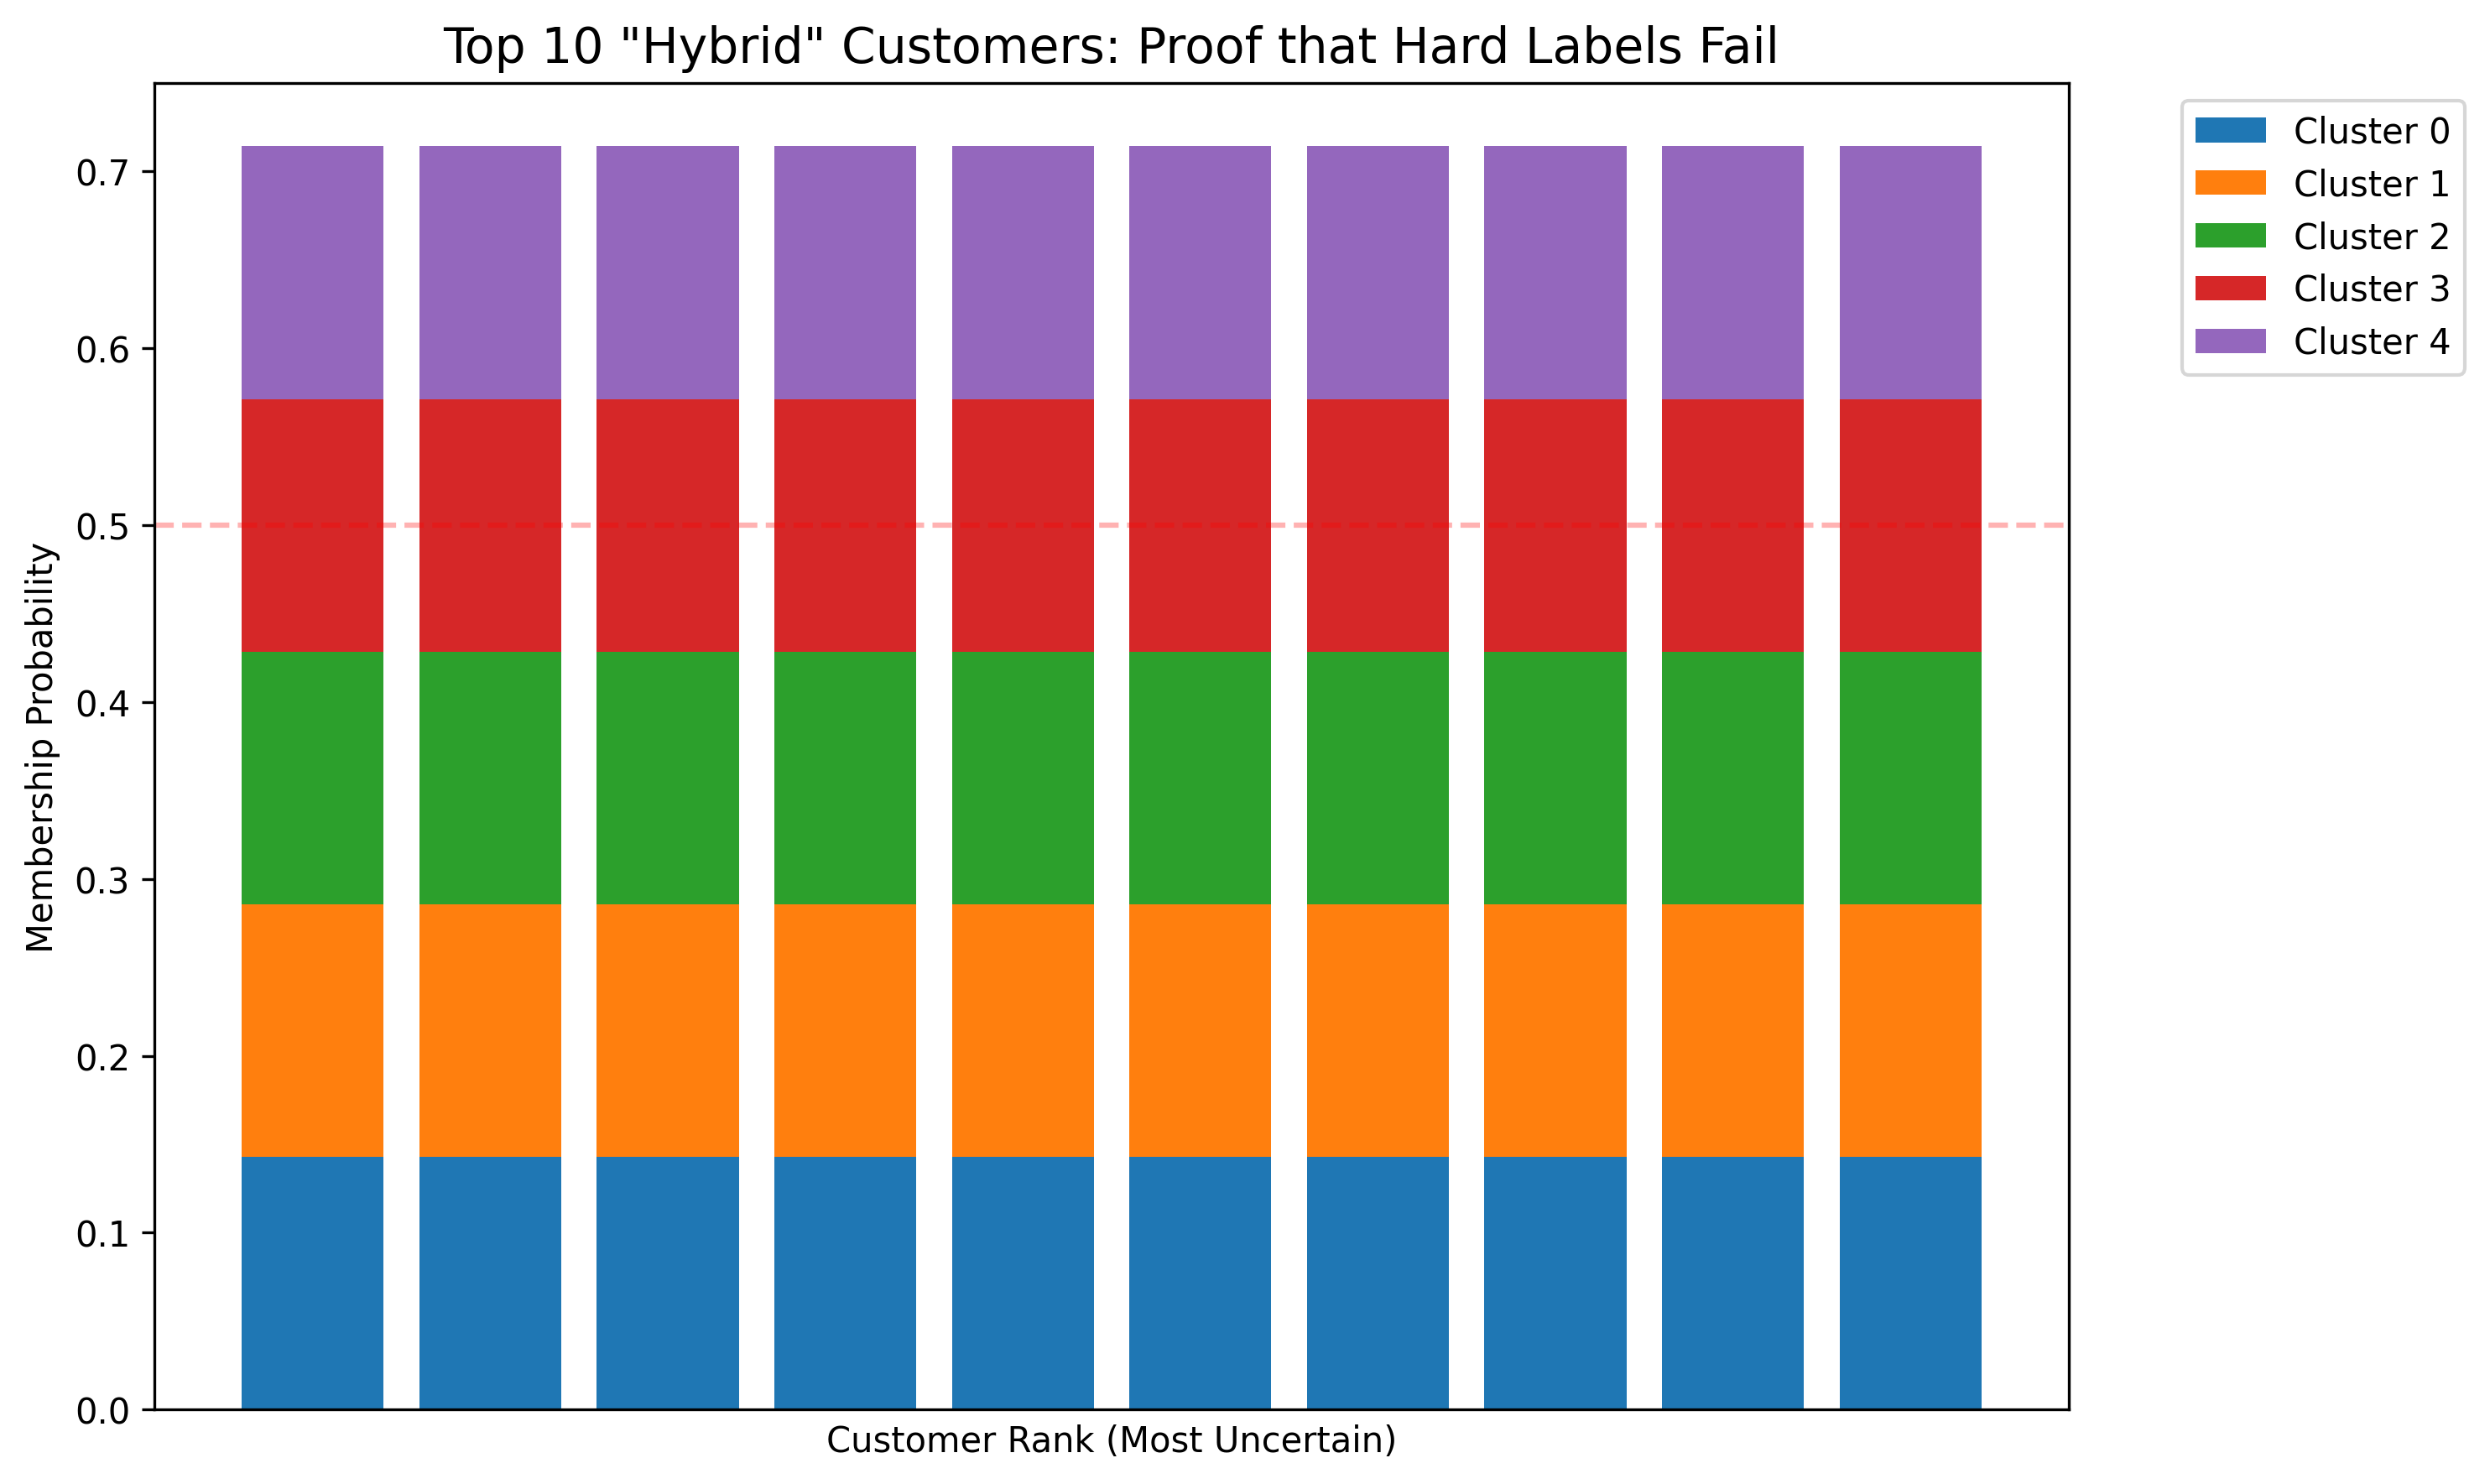
\includegraphics[width=1.0\textwidth]{charts/top10hybrid_customers.png}
    \caption{Top 10 Hybrid Customers. Each bar represents a customer; the colored segments show their probability of belonging to different clusters.}
    \label{fig:hybrid}
\end{figure}

\section{Conclusion}
Fuzzy clustering offers a powerful alternative to hard clustering for customer segmentation. By acknowledging that customers often exhibit multi-segment characteristics, businesses can identify "hybrid" users and design more targeted strategies. The experimental results confirm that a significant portion of the customer base (approx 35\%) lies in transitional zones, which C-Means fails to capture effectively.

\bibliographystyle{plain}
\bibliography{references} 
\end{document}